\documentclass[sigconf]{acmart}
\settopmatter{printfolios=true}

% = = = ACM Metadata
%\setcopyright{acmcopyright}
%\copyrightyear{2018}
%\acmYear{2018}
\acmDOI{10.1145/3478431.3499378}
\acmConference[SIGCSE '22]{The 53rd ACM Technical Symposium on Computer Science Education}{March 2--5, 2022}{Providence, RI}
%\acmBooktitle{SIGCSE 2022 – 53rd ACM Technical Symposium on Computer Science Education, March 2--5, 2022, Providence, RI}
%\acmPrice{15.00}
%\acmISBN{978-1-4503-XXXX-X/18/06}
%%\acmSubmissionID{123-A56-BU3}

% = = = Latin Short-forms (ie, eg, etc, et al)
\usepackage{xspace}
\newcommand{\etal}{\textit{et al.}\xspace}
\newcommand{\etc}{\textit{etc.}\xspace}
\newcommand{\ie}{\textit{i.e.,}\xspace}
\newcommand{\eg}{\textit{e.g.,}\xspace}
\newcommand{\cf}{\textit{cf.}\xspace}
\newcommand{\supra}{\textit{Supra}\xspace}
\newcommand{\nee}{\textit{n\'ee}\xspace}

% = = = Colored text (textblue)
\newcommand{\textblue}[1]{\textcolor{blue}{#1}}


% = = = Top Matter

\begin{document}

\title{Opening sentences in academic writing}
\subtitle{How security researchers defeat the blinking cursor}

\author{Didem Demirag}
\affiliation{\institution{Concordia University} \city{Montreal} \state{QC} \country{Canada}}
\email{d_demira@encs.concordia.ca}
\author{Jeremy Clark}
\affiliation{\institution{Concordia University} \city{Montreal} \state{QC} \country{Canada}}
\email{j.clark@concordia.ca}

\begin{abstract}

Traditionally, education in computer science focuses on stakeholders like teachers, undergraduate students, and employers. However researchers also educate themselves about recent results and new subject matters. An important vehicle in this informal, self-education process is reading peer-reviewed academic papers---papers that are also used in the curriculum of graduate-level research courses. Technical writing skills are important in this domain, as well as engaging the reader with interesting text. This paper is a study of academic writing. We study in depth the first sentence used by researchers in opening their academic papers and how this sentence operates to draw the reader in. We use a corpus of 379 papers from a top-tier cybersecurity conference and use qualitative analysis (coding from grounded theory) to create a taxonomy of 5 general types and 14 sub-types of opening sentences. In this paper, we define and illustrate each type through examples, and reflect on what we learned about writing after examining all of these sentences.

\end{abstract}

\begin{CCSXML}
<ccs2012>

   <concept>
       <concept_id>10003456.10003457.10003527.10003528</concept_id>
       <concept_desc>Social and professional topics~Computational thinking</concept_desc>
       <concept_significance>500</concept_significance>
       </concept>
       <concept>
<concept_id>10003456.10003457.10003527.10003538</concept_id>
<concept_desc>Social and professional topics~Informal education</concept_desc>
<concept_significance>500</concept_significance>
</concept>
   <concept>
       <concept_id>10002978.10003006</concept_id>
       <concept_desc>Security and privacy~Systems security</concept_desc>
       <concept_significance>300</concept_significance>
       </concept>
 </ccs2012>
\end{CCSXML}

\ccsdesc[500]{Social and professional topics~Informal education}
\ccsdesc[500]{Social and professional topics~Computational thinking}

\keywords{Scientific Writing, Education, Cybersecurity}

\maketitle

\section{Introductory Remarks}

What makes the writing style of an academic paper stand out? Strong technical writing is partially founded on \textit{SIGCSE} research dating back to the 1990s on how to move writing from the English department into computer science~\cite{Pes91,TP93,FPC96,Kay98}. Technical writing is now considered a necessary communication skill in our curriculum (\cf \textit{ACM/IEEE Computing Curricula 2020}~\cite{CC2020,CC2020report}).

In a departure from many \textit{SIGCSE} papers, educators in our work are not teachers in a classroom but are authors of academic papers who transfer knowledge to their readers. A well-written paper can reach a wide audience beyond conference attendees and others who benefit from direct communication with the authors. Further, academic papers are used in the classroom, particularly in courses offered to graduate students. For a paper to be effective, it must first catch the attention of the course instructor and then engage the interest of the students. While most researchers are, or were, students, and writing is included in modern curricula, writing research papers is an advanced form of writing considered too ambitious for teaching to undergraduates~\cite{Gar10}. Therefore, crafting academic papers is often self-taught and/or passed from supervisors to students through mentorship~\cite{Mir11}.

Writing tools and systems help produce competent text, but tend not to enhance elegance and style. If writing style is difficult to teach and analyze, what can be done? In this paper, we build a `zoo' of writing samples (conceptualized by Miro~\cite{Mir11} at \textit{SIGCSE'11}), placed in a taxonomy we develop, to exhibit different writing styles for writers and readers to study and learn from. The specific lessons drawn from viewing our zoo are meant to be subjective, and depend on the viewer's personal context. A secondary contribution of our paper is our methodology for building a zoo. We hope to see this applied to other domains of writing.

Our methodology is empirical and positive. To illustrate what we mean, consider a research paper that designs and tests a pedological tool in an educational setting. By contrast, an \textit{empirical} paper might survey a set of courses from around the world. Often before a \textit{normative} approach (\ie what ought to be done) can be formulated, it is instructive to first consider a \textit{positive} approach (what is being done). Our zoo is not a curation of `good' writing samples (beyond being acceptable for publication in a top-tier conference) but offers a large set of samples that are carefully organized by our interpretation of what the writers intended to convey.

\paragraph{The Opening Sentence}

We believe it is fruitful to study the writing style of academic computer science articles at different levels of granularity. As a general trade-off, short writing samples enable the study of a large number of samples, while longer writing samples enable a broader representation of the writing style. In this work, we choose to look at a large number of very short samples---each only a single sentence. In choosing which sentence to study from each paper, the first sentence is an intuitive candidate. The opening sentence of a paper needs to be bold, convey the importance of the subject of the paper, and hook the reader. The novelist Stephen King is said to spend ``months or even years'' writing an opening sentence~\cite{Fas13}. The academic Steven Pinker notes that,

\begin{quote}
``Good writing starts strong. Not with a cliché (`Since the dawn of time’), not with a banality (`Recently, scholars have been increasingly concerned with the question of …’), but with a contentful observation that provokes curiosity.''~\cite{Pin15}
\end{quote}

In this paper, we study the opening sentences of 379 papers from the field of information systems security. We use a variant of grounded theory~\cite{glaser1968discovery} to classify the opening sentences of each of these papers according to what the sentence is doing to advance an argument and engage with the reader. For example, a paper might start with a historical fact, argue the importance of the subject, tell a story, or open with a question (as this paper itself does). We develop 5 main categories, with 14 sub-types in total. We provide many examples of each and a guide to distinguishing them---an opening sentence `zoo.' Such a set of examples, called a zoo by Miro in \textit{SIGCSE`11}, is suggested for students to develop style and taste (beyond competence) in writing~\cite{Mir11}.

\paragraph{Source Data} Before initiating our work, we were unsure if it would be possible to understand the opening sentences of academic papers without some domain knowledge of the field (we discuss our conclusions on this in Section~\ref{sec:disc}). Thus we made the initial decision to look at papers from our own research area: security.

The field of security has hundreds of conferences and workshops but is recognized as having four top conferences (as ordered within a calendar year): \textit{The Network and Distributed System Security Symposium (NDSS)}, \textit{IEEE Symposium on Security and Privacy}, \textit{USENIX Security Symposium}, and \textit{ACM Conference on Computer and Communications Security (CCS)}. These conferences have considerable overlapping authors\footnote{System Security Circus 2020: \url{http://s3.eurecom.fr/~balzarot/notes/top4}} and program committee members, and we hypothesize (but did not test) that the analysis would be invariant to which conference the papers came from.

We selected \textit{USENIX Security}, which has always offered its proceedings as open access, allowing us to side-stepping any potential copyright issues with opening our dataset and work. It also offers its proceedings in formats that were useful for our project: \ie all papers in a single file; and \texttt{epub} format in addition to \texttt{pdf}. We used three consecutive years (2014--2016) for a total of 379 papers. We analysed every opening sentence from the main body of the paper (as opposed to the abstract, which we view as serving an archival role for the paper).

	\paragraph{Open Access} Our raw data, the full set of original papers, and the full set of our codes are available as an NVIVO database on a public GitHub repository.\footnote{GitHub: \url{https://github.com/MadibaGroup/2020-Opening}}

\section{Preliminaries and Related Work}



\paragraph{Opening Sentences.}

Our idea to examine opening sentences came from Pinker's style guide~\cite{Pin15}, which is devoted in part to improving technical, scientific, and academic writing. Pinker also devotes a section of the book to the role of the opening sentences of a work (illustrating with popular non-fiction books). When we reflected on our own difficulty with `getting a paper going,' we conceived of this project. To our knowledge, opening sentences have not been systematically categorized before. In an older paper, King looks at opening sentences in medical research~\cite{king1967opening}. The article provides stylistic advice---draw the readers' attention, be concise and clear about stating the main theme of the paper---and he gives examples from medical writing and explains different ways to simplify overcomplicated sentences by shortening them. By contrast, our paper is not normative at all (it is not on how to improve an opening sentence) but is instead a neutral classification of how others have decided to open their papers, looking for trends and the variations in approach.

\paragraph{Academic Writing.}  Miro at \textit{SIGCSE'11}  presents a set of falsifiable writing principles to make good writing similar to engineering~\cite{Mir11}. For example, principles at the granularity of a single sentence include: `put known information at the beginning of a sentence and new, important information at the end;' `sentences begin and end well;' and `each sentence exposes only one idea' (note these are for any sentence, and not restricted to an opening sentence). However Miro considers style---personality and enjoyment---as beyond these principles. Instead, he suggests building a `zoo' of writing exemplars for students to study, process, and reflect on. Our paper strives to build such a zoo for opening sentences.

Côté and Custeau~\cite{CC92} describe in the \textit{SIGCSE Bulletin} an evaluation method for grading a student's article (part of a pedagogical exercise they are testing) along 23 criteria: \eg `the topic is pertinent, original, and interesting;' `redundancy adds to clarity;' and `references are made in the text to illustrations.' In our work, we choose one of their criteria for in-depth study: `\textbf{the introduction draws attention and is interesting to read}.' Future work might adapt our methodology for studying other criteria.

%Outside of computer science, Cameron \etal explains the struggles of the writing process and suggests strategies to helps novice writers to overcome them~\cite{cameron2009demystifying}. Hartley presents a bilingual study on improving different aspects of academic writing in psychology to increase readability~\cite{hartley2012new}. Biber \etal discuss stereotypical characteristics of academic writing including complex grammar structures~\cite{biber2010challenging}; a theme of Pinker's book as well~\cite{Pin15}.

\paragraph{Grounded Theory.} Grounded theory is an analysis method for qualitative data~\cite{glaser1968discovery}. In grounded theory, one or more practitioners will examine the data to divisions between different concepts. The data is then partitioned at these points and concepts are labeled with a code. By performing coding, the aim is to come up with new high-level theories and concepts at the end of the process. Coding is an iterative process and several rounds of coding can be performed to refine the categories. At the end of the process, a new theory that is based on the data is presented. 

%Grounded theory is used as a methodology in security and privacy research. Some examples include: user mental models of cryptocurrency systems~\cite{mai2020user}, how blockchain technology is perceived and how it is used~\cite{ruoti2019blockchain}, preferences for security warning types~\cite{danilova2020one}, the factors that influence software developers' motivation towards security~\cite{assal2018motivations},  how users manage their online security posture~\cite{ruoti2017weighing}, and how users manage their passwords~\cite{stobert2014password}.

\section{Categorization}
\label{sec:categories}

	\begin{figure*}[t]
	\centering
	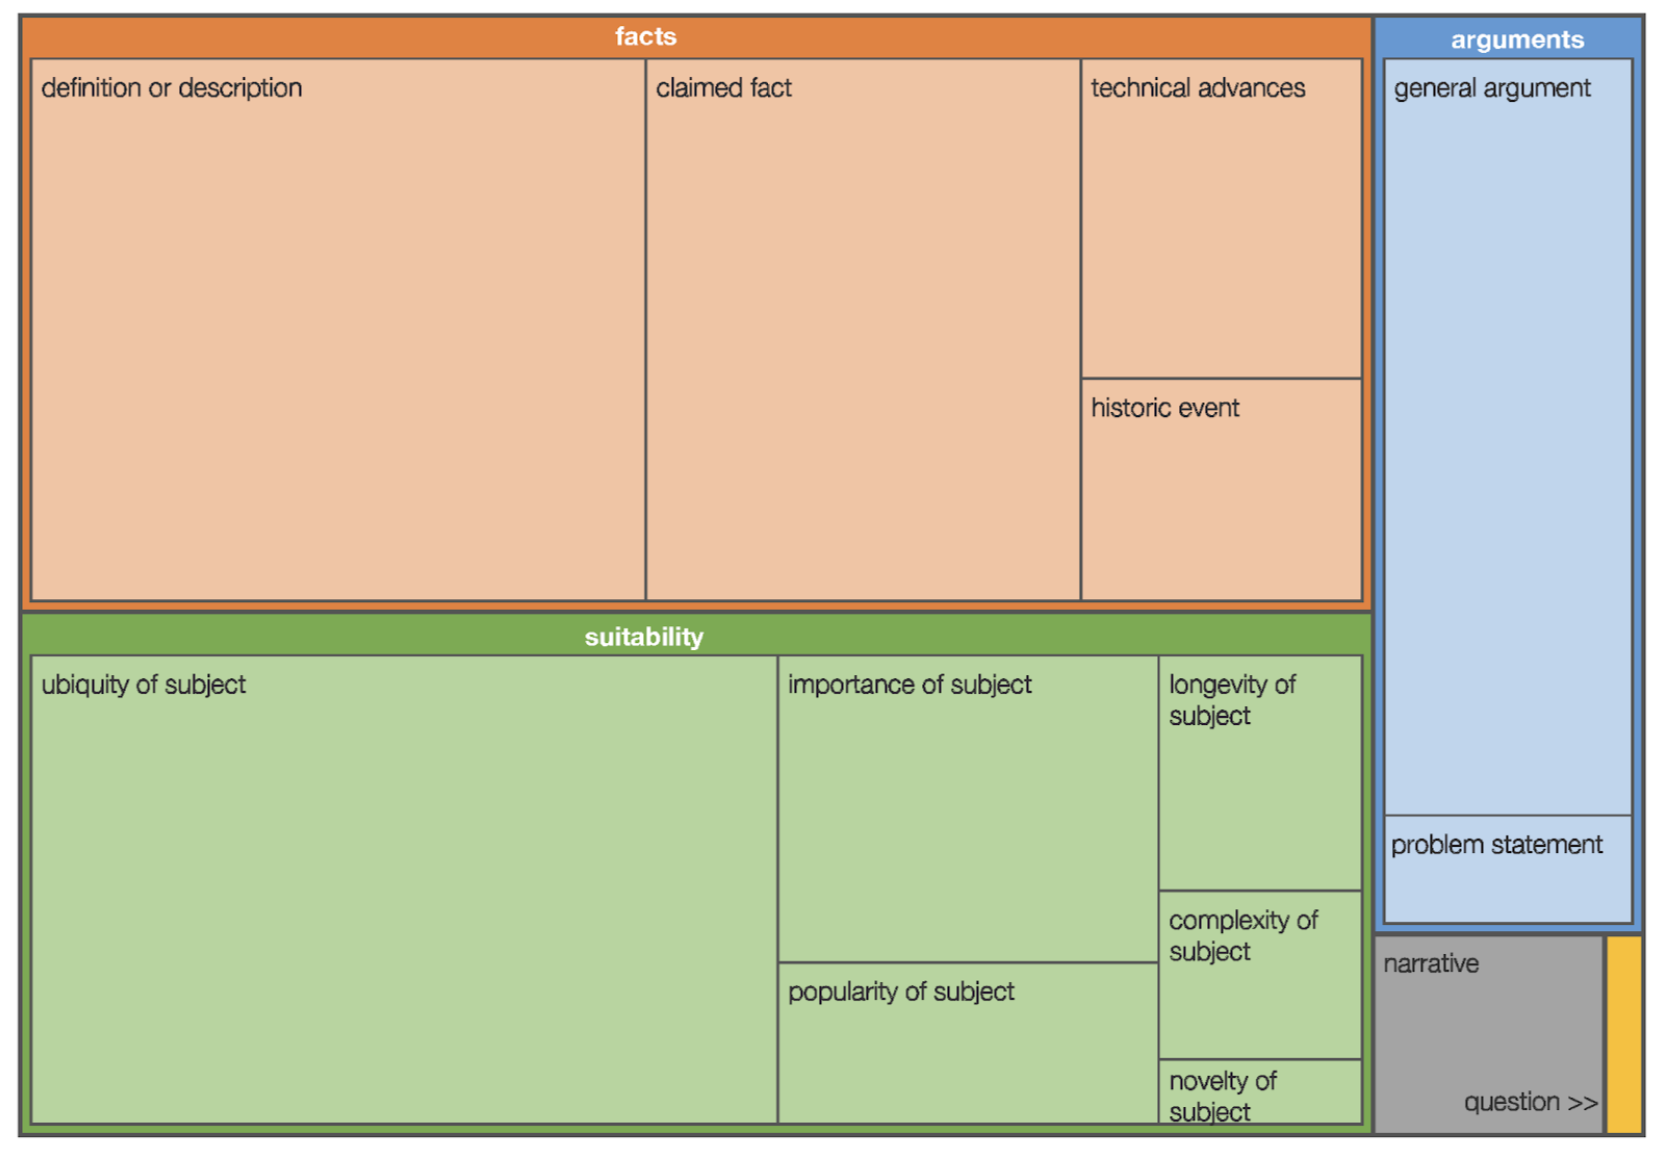
\includegraphics[width=0.7\textwidth]{image.png}
	\caption{A treemap of our codes for the opening sentences of 379 research papers. The size (in area) of each visualized code is proportional to the number of sentences with that code.\label{fig:treemap}}
	\end{figure*}

	Figure~\ref{fig:treemap} shows the taxonomy of our codes where the area of the box is proportional to how many times they were used. We provide a description of each category, as well as several examples.

\paragraph{Methodology.}

To arrive at this figure, we followed the coding techniques of grounded theory assisted by the qualitative analysis software tool NVIVO. To start, one of us partitioned out the opening sentence of each paper, which also anonymized the writing samples. Together, we read dozens of sentences without coding and establish a guiding principle: to code what the authors are trying accomplish; not just the content, but the intension of the sentence.

For the first year of proceedings, both of us `open coded' the papers together to establish an initial codebook. For the following two years of proceedings, one of us coded and the other reviewed, discussing and resolving disagreements together. If more than one code applied to a sentence, we sought the best fit and avoided coding a sentence with more than one code.

Periodically, we reviewed the codebook itself together. First, we would look at the codes themselves (as opposed to the sentences) for relationships (`axial coding'). Second, we looked at all the samples within each specific code to see if they were coherent and to re-code or further sub-divided as necessary (`code upon'). 

%We re-coded any sentences that stuck out as appearing different (should the sentence be coded as something else? Does it require a new code we do not have? Is it actually coded correctly but sticking out for some other reason?).

%For example, we initially had a disproportionate number of suitability arguments so we looked very closely at each sentence to tease out distinctions in what the argument was based on (\eg the subject is suitable for research because it has been studied for a long time, has not been studied at all, is popular now, is in use by many people, \etc).

%Examining at all the samples in a single code also helped us with quality control, ensuring the samples are all coherent with each other.

We halted after coding the third year of proceedings, as we determined that the newest samples did not substantially modify our codebook (\ie in terms of sub-categorizing, reclassifying or creating new codes) or the proportion of samples in each code. We did not measure this explicitly but relied on our judgement. The final step of grounded theory is to pull general theories out of the codes and their categorization, which we did not pursue since our end goal was classification. Thus we use the coding techniques of grounded theory rather than exactly grounded theory itself. %We also were not coding the \textit{content} of the sentences, only the kind of writing they exhibit. For these reasons, we emphasize that we used the coding techniques of grounded theory rather than exactly grounded theory itself.

\paragraph{Replication, Validity \& Extension.}

A replication of our study (starting with the same writing samples) has some potential of producing different results. Starting with the codebook itself, we expect the codes would be named differently, the spectrum between objective fact and subjective argument can be sub-divided differently, and the fidelity of sub-categorization of codes might also differ. However we expect the highest-level intentions (facts, arguments, narratives, \etc) should be conveyed in any open coding of the samples, and should a a study start with our codebook, we are confident the classification of the samples themselves would not deviate significantly.

We encourage researchers to use our methodology to build zoo's for other writing domains. For close domains (\eg other CS disciplines), we would advise skipping the open coding step, and use our codebook directly. It is quite general and appears applicable to different forms of persuasive writing. Of course, during coding, researchers should revisit the codebook and use axial coding and code upon techniques to customize the codebook as necessary. It would be interesting to compare zoos across disciplines (within and outside of CS), across languages, and author demographics.

\paragraph{Note on Quotations.} Quoted sentences are presented verbatim. When the quoted sentence includes a citation, we leave the citation intact. Thus that citation will not be found in the bibliography of our paper, but can be found by looking at the paper being quoted.

	\subsection{Facts}
	\subsubsection{Facts: Definition or Description}




	Many papers start with a straightforward definition of the subject of the paper. These tend to be neutral and like something you would read in a glossary.

	\begin{itemize}

		\item	``Malware sandboxes are automated dynamic analysis tools that execute samples in an isolated and instrumented environment.''~\cite{graziano2015needles}

		\item	``Secure two-party computation allows two parties to process their sensitive data in such a way that its privacy is protected.''~\cite{demmler2014}

		\item	``HMAC is a cryptographic authentication algorithm, the ‘Keyed-Hash Message Authentication Code,’ widely used in conjunction with the SHA-256 cryptographic hashing primitive.''~\cite{beringer2015verified}

	\end{itemize}

	Similarly, papers might provide a description of what the subject of a sentence does or how it works. These are also neutral statements and like something you’d read in a textbook.

	\begin{itemize}

		\item	``Traditionally, digital investigations have aimed to recover evidence of a cyber-crime or perform incident response via analysis of non-volatile storage.''~\cite{saltaformaggio2014dscrete}

		\item	``Mobile social applications discover nearby users and provide services based on user activity (what the user is doing) and context (who and what is nearby).''~\cite{lentz2014sddr}

		\item	``To reduce the memory footprint of a system, the system software shares identical memory pages between processes running on the system.''~\cite{yarom2014flush+}
	\end{itemize}
	\subsubsection{Facts: Claimed Fact}

	Another neutral approach to an opening sentence is to provide a fact that is relevant to the subject of the paper. Later we will discuss arguments which are often expressed as if they are facts but are only debatably true. A claimed fact’s correctness should either be apparent or at least provable (i.e., falsifiable).
	\begin{itemize}
		\item	``Users are often advised or required to choose passwords that comply with certain policies.''~\cite{komanduri2014telepathwords}

		\item	``Mobile apps frequently demand access to private information.''~\cite{tripp2014bayesian}

		\item	``For several decades, car keys have been used to physically secure vehicles.''~\cite{garcia2016lock}
	\end{itemize}
	Some sentences use stronger and more vivid language but are still factually based.
	\begin{itemize}
		\item	``In spite of extensive industrial and academic efforts (e.g., [3, 41, 42]), distributed denial-of-service (DDoS) attacks continue to plague the Internet.''~\cite{fayaz2015bohatei}
	\end{itemize}

	\subsubsection{Facts: Technical Advances}

	Many opening sentences lay out a technical advance in the subject of the sentence. This creates a window of opportunity for the researcher to later identify a novel research problem caused by the changing technology.  It is common to see words like: evolve, become, transition, and improve.
	\begin{itemize}
		\item	``Recent advances in cloud computing enable customers to outsource their computing tasks to the cloud service providers (CSPs).''~\cite{pattuk2014preventing}

		\item	``Browsers have evolved over recent years to mediate a wealth of user interactions with sensitive data.''~\cite{jagpal2015trends}

		\item	``Since its beginning in the early nineties, the Web evolved from a mechanism to publish and link static documents into a sophisticated platform for distributed Web applications.''~\cite{lekies2015unexpected}
	\end{itemize}
	\subsubsection{Facts: Historic Events}

	A final type of neutral opening sentence will refer to some historic event.
	\begin{itemize}
		\item	``In 1996, Wagner and Schneier performed an analysis of the SSL 3.0 protocol [67].''~\cite{van2016request}

		\item	``In February 2011, a new Tor hidden service [16], called “Silk Road,” opened its doors.''~\cite{soska2015measuring}

		\item	``The Network Time Protocol (NTP) is one of the Internet’s oldest protocols, dating back to RFC 958 [15] published in 1985.''~\cite{dowling2016authenticated}
	\end{itemize}
	In some cases, a paper opens with a “compound” sentence that makes reference to a historic event in one clause of the sentence, while having additional clauses of a different category. For example, the following sentence refers to a historic event as well as a technical advance.

	\begin{itemize}
		\item 	``Starting from Denning’s seminal work in 1986 [9], intrusion detection has evolved into a number of different approaches.''~\cite{caselli2016specification}
	\end{itemize}

	In our analysis, some sentences are coded with more than one code but we do so sparingly.


	\subsection{Arguments}
	\subsubsection{Arguments: General Argument}

	Many opening sentences issue a subjective argument that represents the authors’ opinion. Unlike a fact, it isn’t straightforward that the reader will accept it as true. While arguments are less neutral than facts, they can be more interesting and provocative, which can help draw the reader into the paper.

	The arguments we categorize under “general arguments” do not fit elsewhere in our categorization system. As we go through more categories, we will see other more specific kinds of arguments.
	\begin{itemize}
		\item ``It is a truth universally acknowledged, that password-based authentication on the web is insecure.''~\cite{li2014emperor}

		\item 	``The dismissal of human memory by the security community reached the point of parody long ago.''~\cite{bonneau2014towards}

		\item ``In recent years, unwanted software has risen to the forefront of threats facing users.''~\cite{thomas2016investigating}

		\item 		``The phenomenal growth of Android devices brings in a vibrant application ecosystem.''~\cite{chen2015finding}
	\end{itemize}


	\subsubsection{Arguments: Problem Statement }

	A special type of argument is a “problem statement” which uses the opening sentence to establish a problem or challenge to be solved.
	\begin{itemize}
		\item ``A key challenge when running untrusted virtual machines is providing them with efficient and secure I/O.''~\cite{smolyar2015securing}

		\item``Determining the semantic similarity between two pieces of binary code is a central problem in a number of security settings.''~\cite{egele2014blanket}

		\item``It is difficult to keep secrets during program execution.''~\cite{rane2015raccoon}

		\end{itemize}
For some sentences, the problem is not stated explicitly but can be inferred from what is said. For example, the “pressure to respond” in the following sentence implies a problem.

\begin{itemize}

		\item ``As popular applications rely on personal, privacy-sensitive information about users, factors such as legal regulations, industry self-regulation, and a growing body of privacy-conscious users all pressure developers to respond to demands for privacy.''~\cite{fredrikson2014zo}
	\end{itemize}


	\subsection{Suitability}
	\subsubsection{Suitability: Importance of subject}

	A large set of sentences make a special kind of argument: that the subject of the opening sentence is suitable or worthy of research. The exact reasons they are suitable fall into a few sub-categories: the subject is important, ubiquitous, complex, novel, popular with other researchers, or has been around a long time.

	Many opening sentences state that their subject is important, with the implication that it is thus suitable for research.
	\begin{itemize}
		\item 	``Security has now become an important and real concern to connected and/or automated vehicles.''~\cite{cho2016fingerprinting}

		\item 	``Error handling is an important aspect of software development.''~\cite{jana2016automatically}

		\item 	``SSL/TLS is, due to its enormous importance, a major target for attacks.''~\cite{meyer2014revisiting}
	\end{itemize}


	Some sentences do not explicitly use the word “important” but find other ways to convey the same notion. For example, a concern or component might be described as essential or crucial or serious.
	\begin{itemize}
		\item 	``The threat of data theft in public and private clouds from insiders (e.g. curious administrators) is a serious concern.''~\cite{dinh2015m2r}

		\item 	``The same-origin policy (SOP) is a cornerstone of web security, guarding the web content of one domain from the access from another domain."~\cite{zheng2015cookies}
	\end{itemize}


	\subsubsection{Suitability: Ubiquity of subject}

	The most popular kind of opening sentence argues that a subject is suitable for research because it is ubiquitous and widely used.
	\begin{itemize}
		\item ``Billions of users now depend on online services for sensitive communication.''~\cite{melara2015coniks}

		\item	``Embedded systems are omnipresent in our everyday life.''~\cite{costin2014large}

		\item	``Android is the major platform for mobile users and mobile app developers.''~\cite{oltrogge2015pin}
	\end{itemize}


	\subsubsection{Suitability: Popularity of subject}

	While the ubiquity of a subject corresponds to how widely it is used, a closely related variant points out that the subject has received a lot of attention. Often, this means attention from other researchers which lends credibility to the subject for further research.
	\begin{itemize}
		\item	``Protecting the privacy of user data within mobile applications (apps for short) has always been at the spotlight of mobile security research.''~\cite{nan2015uipicker}

		\item	``The black-market economy for purchasing Facebook likes, Twitter followers, and Yelp and Amazon reviews has been widely acknowledged in both industry and academia [6, 27, 37, 58, 59].''~\cite{viswanath2014towards}

		\item	``Since the first widely-exploited buffer overflow used by the 1998 Morris worm [27], the prevention, exploitation, and mitigation of memory corruption vulnerabilities have occupied the time of security researchers and cybercriminals alike.''~\cite{di2015elf}
	\end{itemize}
	\subsubsection{Suitability: Longevity of subject }

	In this category, how long a subject has been around is the key component to why it is a suitable subject for study. In some cases, a specific duration is provided and in others, it is implied that the amount of time is significant.
	\begin{itemize}
		\item ``Redaction of sensitive information from documents has been used since ancient times as a means of concealing and removing secrets from texts intended for public release.''~\cite{araujo2015compiler}

		\item	``Since its beginning in the early nineties, the Web evolved from a mechanism to publish and link static documents into a sophisticated platform for distributed Web applications.''~\cite{lekies2015unexpected}
	\end{itemize}


	\subsubsection{Suitability: Complexity of subject}

	In this category, the complexity of the subject is highlighted, implying that the complexity creates new issues or requires further research. The complexity might be inherent to the subject itself. Or there might be a complex set of external factors to consider.
	\begin{itemize}
		\item 	``Today, large and complex software is built with many components integrated using APIs.''~\cite{yun2016apisan}

		\item ``The capabilities and limitations of disassembly are not always clearly defined or understood, making it difficult for researchers and reviewers to judge the practical feasibility of techniques based on it.''~\cite{andriesse2016depth}

		\item 	``As popular applications rely on personal, privacy-sensitive information about users, factors such as legal regulations, industry self-regulation, and a growing body of privacy-conscious users all pressure developers to respond to demands for privacy.''~\cite{fredrikson2014zo}
	\end{itemize}


	\subsubsection{Suitability: Novelty of subject}

	Finally, a degree of novelty is an important component in any research question so it is unsurprising that papers begin arguing novelty from their opening sentence. In this category, sentences focus on something that is new or emerging.
	\begin{itemize}
		\item 	``In the last few years, a new class of cyber attacks has emerged that is more targeted at individuals and organizations.''~\cite{le2014look}

		\item  ``Although the operating system (OS) kernel has always been an appealing target, until recently attackers focused mostly on the exploitation of vulnerabilities in server and client applications— which often run with administrative privileges—as they are (for the most part) less complex to analyze and easier to compromise.''~\cite{kemerlis2014ret2dir}
	\end{itemize}

	This sentence manages to appeal to both longevity and novelty by relating two subjects.
	\begin{itemize}

		\item  ``While cryptocurrency has been studied since the 1980s [22, 25, 28], bitcoin is the first to see widespread adoption.''~\cite{heilman2015eclipse}

	\end{itemize}

	\subsection{Narrative}

	A potentially interesting way to draw a reader into a paper is by establishing a narrative: a scenario that gets the reader thinking about themselves or other people and what they might do.
	\begin{itemize}
		\item 	``Consider that you are a domain owner, holding a few domain names that you do not have a better use of.''~\cite{alrwais2014understanding}

		\item 	``Consider the setting where a client owns a public input x, a server owns a private input w, and the client wishes to learn z := F(x,w) for a program F known to both parties.''~\cite{ben2014succinct}
	\end{itemize}

	Narratives might also set a scene, like the academic version of an establishing shot from films and TV.

	\begin{itemize}

		\item 	``Our phones are always within reach and their location is mostly the same as our location.''~\cite{michalevsky2015powerspy}

		\item 	``We live in a “big data” world.''~\cite{lecuyer2014xray}

		\item 	``The battle for the living room is in full swing.''~\cite{oren2014aether}
	\end{itemize}


	\subsection{Question}

	Making the reader curious is another good way to begin a paper, and this can be accomplished using a question. In our sample, this was underused with only one example.
	\begin{itemize}
		\item ``Do programmers leave fingerprints in their source code?''~\cite{caliskan2015anonymizing}
	\end{itemize}


	\section{Discussion}
	\label{sec:disc}


	\paragraph{Domain Expertise.} We pondered whether we could apply our analysis to a domain in which we were not experts. Obviously a non-expert in security would not understand the technical content of many of our sentences, but would they be able to tell the difference between, say, a historic fact and a suitability argument?

	We are unsure but skeptical. Consider the following sentence: ``The widespread adoption of DEP, which ensures that all writable pages in memory are nonexecutable, has largely killed classic code injection attacks''~\cite{carlini2014rop}. A non-expert who is unfamiliar with DEP or code injection could understand the gist of the sentence: code injection is an \textit{attack}, therefore it is \textit{bad}; DEP is \textit{good} because it reduces something that is bad. But what if the authors of the sentence had dropped the word `attack' and instead simply ended: ``DEP\ldots has largely killed classic code injection.'' Now it is ambiguous to a non-expert whether DEP is good or bad, in fact the strength of the word `kills' might lead the non-expert to conclude DEP is bad. While most sentences are not like this, we see this as evidence that our analysis should be undertaken by domain experts and not general readers.

	\paragraph{Sentence Length.} We examined the shortest and longest sentences in our dataset. Short sentences are striking and easy to remember. The shortest ones from our data set were four words long: ``Video is ineffably compelling''~\cite{brocker2014iseeyou} and ``Software bugs are expensive''~\cite{rebert2014optimizing}. Long sentences can obviously convey more information or make a complex argument, but they might have to be read a few times to fully parse what they are saying. King has a similar argument in~\cite{king1967opening}, where he gives an example of a long opening sentence in medical writing and he simplifies the sentence by shortening it and as a result making it more concise and easier to parse.

	\paragraph{Security-specific Approach.} There was one set of sentences that usually fell under the \textit{suitability: importance of subject} code that was very specific to security. In security, it is important to researchers to tackle the biggest threats. Many use their opening sentence to position themselves as doing so. Many of them flatly state that their research area is the most prevalent threat (``In recent years, unwanted software has risen to the forefront of threats facing users''~\cite{thomas2016investigating}; ``Today, runtime attacks remain one of the most prevalent attack vectors against software programs''~\cite{davi2014stitching}; ``Remote malware downloads currently represent the most common infection vector'~\cite{nelms2015webwitness}). Some prefer to make their point in a stronger way with a colourful choice of words (``In spite of extensive industrial and academic efforts (e.g., [3, 41, 42]), distributed denial-of-service (DDoS) attacks continue to plague the Internet''~\cite{fayaz2015bohatei}). We look at colourful sentences next, with another example using the word `plague.'

	\paragraph{Colour} We also analyzed to what extend the authors add `colour commentary' in the opening sentence. The decision to use this type of commentary is related to how researchers perceive and define the seriousness of their topic. Is avoiding all colour in the text a way to prove that the problem is significant and should be taken seriously? Or should writers add some colour to make the writing more engaging and easier to hook the reader? Examples of sentences that use a more vivid choice of words include: ``The defacement and vandalism of websites is an attack that disrupts the operation of companies and organizations, tarnishes their brand, and plagues websites of all sizes, from those of large corporations to the websites of single individuals''~\cite{borgolte2015meerkat}; ``The dismissal of human memory by the security community reached the point of parody long ago''~\cite{bonneau2014towards}; ``Video is ineffably compelling''~\cite{brocker2014iseeyou}.

	Using colourful language is probably best in moderation. Text that is very ornate and elaborate is deridingly called `purple prose.' We did not find any examples in our data set, but to what extent is this a reflection of writing in information technology? An interesting area of future work is to examine the usefulness of our taxonomy in both other STEM domains, but also in academic writing in arts and the humanities.

	\paragraph{The Arc of Time.} Appealing to the notion that a domain is important because of its longevity is also a common way to start a paper in our data set. The idea of appealing to years or decades of work is extremely common (``Over the last few years there have been numerous reports…''~\cite{nakibly2016website}; ``The last decade in cryptography…''~\cite{alkim2016post}; ``Over the past few years, face authentication systems…''~\cite{xu2016virtual}; ``For several decades, car keys…''~\cite{garcia2016lock}). The longest timeframe in our dataset is: ``Redaction of sensitive information from documents has been used since ancient times as a means of concealing and removing secrets from texts intended for public release''~\cite{araujo2015compiler}.

	\section{Conclusion}

	We hope that our results are interesting, but that they also raise consciousness of thoughtful writing in research papers. 
As researchers ourselves, we have often found ourselves staring at a blinking cursor, trying to come up with a compelling way to start our paper. After completing our analysis, we find ourselves proactively choosing how to start our writing. The zoo also allows us to try on different approaches (\eg `what if we started with a narrative instead of the importance of the domain?') to find one that works. Finally, we may not have fully answered the question we started with (`what makes writing style stand out?') but we have equipped readers with a set of samples to examine while asking themselves this question. 
	
	%We have noted that the education of information technology and computer science (\eg SIGITE and SIGCSE) domains have a blindspot for technical writing skills when it comes specifically to research papers. We hope to instigate research in this area given the important role that papers play in allowing experts to educate other experts, as well as in the training of students.

	% A bad opening sentence...
	
\begin{acks} 

The \textit{SIGCSE} reviews were thoughtful, insightful, and enthusiastic---thank you to the reviewers. J. Clark acknowledges partial funding of this project from NSERC. 
\end{acks}


	\bibliographystyle{ACM-Reference-Format}
	\bibliography{acmart,papers}

\end{document}

%%
%% End of file `sample-sigconf.tex'.
